\documentclass[10pt,a4paper,UTF8]{article}
\usepackage{zclorg}
\author{Eastern(ZCL)}
\date{}
\title{Matlab与C混合编程}
\hypersetup{
 pdfauthor={Eastern(ZCL)},
 pdftitle={Matlab与C混合编程},
 pdfkeywords={matlab communication simulation C},
 pdfsubject={本文描述LTE-FDD和TDD的频带资源},
 pdfcreator={Emacs 25.0.50.1 (Org mode 8.3.2)}, 
 pdflang={English}}
\begin{document}

\maketitle\xiaosihao
\tableofcontents\newpage\newpage


\section{引言}
\label{sec:orgheadline1}


matlab是Mathworks公司推出的一款强大的仿真软件。由于其简单易用,建模迅捷,函数库保罗万象,因此得到广泛使用,尤其在通信与信息系统仿真中更是大显身手。matlab使用的语言也叫matlab,是一门脚本语言。脚本语言的特性决定了其编写方便快速,但是运行速度却不及C/C++等编译型语言。为综合脚本语言和编译型语言的优点,matlab支持与C的混合编程。本文是我的matlab与C混合编程系列博文的第一篇,主要介绍matlab如何调用C语言编写的函数。在之后的一些博文中介绍matlab提供的调用C函数需要使用的API。

这一系列博文的诸多例子来自matlab自带的帮助文档。在学习的过程中,结合自己的心得,成此博文。读者完全可以通过matlab的帮助文档来学习如何使用这些API。但matlab的帮助文档略显生硬,有些冷冰冰。在涉及重点以及可能会碰到的bug时,不会像我在这里大声疾呼:"这是个坑,小心"。因此我认为这些博文还是有其存在的价值。当然,我也力图博文朗朗上口,深入浅出,读起来引人入胜。

\section{使用mex编译c函数}
\label{sec:orgheadline7}


我们知道在C语言编程过程中,每一个程序都包含 \texttt{main} 函数。在 \texttt{main}  函数中,我们可以调用我们编写的其他函数。如果要在matlab脚本中调用c函数,需要一个特殊的函数将用户自己定义的函数封装起来。这个函数叫做 \texttt{mexFunction} , \texttt{mexFunction} 就像一座桥梁一样链接了matlab脚本语言和C这种编译型语言,matlab调用 \texttt{mexFunction} , \texttt{mexFunction} 调用用户自定义的函数。接下来用一个简单的例子演示如何使用 \texttt{mexFunction} 将我们定义的函数封装起来以及如何在matlab中调用这个C函数。
\subsection{一个例子}
\label{sec:orgheadline2}


假设我们要实现:一个标量 \(x\)  乘以一个适量 \(\mathbf{Y}\),结果保存在矢量 \(\mathbf{Z}\)中。整个过程如式\ref{eq:scalartimevector}所示。
\begin{equation}
\label{eq:scalartimevector}
\mathbf{Z} = x\mathbf{Y}
\end{equation}

我们用C语言实现这个功能,函数命名为 \texttt{arrayProduct} ,代码如下(这个例子就来自matlab的帮助文档):
\lstset{language=C,label= ,caption= ,captionpos=b,numbers=left}
\begin{lstlisting}
void arrayProduct(double x, double *Y, double *Z, int n)
{
  int i;

  for (i=0; i<n; i++) {
    Z[i] = x * Y[i];
  }
}
\end{lstlisting}
\subsection{编写源代码}
\label{sec:orgheadline3}


打开matlab编辑器,创建一个新文件,为其添加文件头
\lstset{language=C,label= ,caption= ,captionpos=b,numbers=none}
\begin{lstlisting}
/*
 *arrayProduct.c - example in MATLAB External Interfaces
 *
 * Multiplies an input scalar (multiplier)
 * times a 1xN matrix (inMatrix)
 * and outputs a 1xN matrix (outMatrix)
 *
 * The calling syntax is:
 *
 *              outMatrix = arrayProduct(multiplier, inMatrix)
 *
 * This is a MEX-file for MATLAB.
*/
#include "mex.h"
\end{lstlisting}
以上代码来自matlab的帮助文档,其为我们展示了如何编写一个清新脱俗的文件头。最后一行是调用 C/C++ 函数必须的头文件,其包含了matlab定义的一些API。先把这个文件保存起来,文件名为 \texttt{arrayProduct.c} ,在后面我们用 \texttt{mex} 命令编译的 \texttt{MEX} 文件会自动命名为 \texttt{arrayProduct} 。在matlab的脚本里调用 \texttt{arrayProduct} 就像调用matlab的内嵌函数一样。对于用户来讲 \texttt{mexFunction} 是透明的,不用关心的。 \texttt{mexFunction} 需要程序员写好,供用户使用,然后程序员深藏功与名,幕后螺丝钉。
\subsection{创建桥梁变量\label{orgtarget1}}
\label{sec:orgheadline4}


这一部分是最重要的,在我学习matlab和c混合编程过程中,这一步用的时间最多。前文曾提到:每一个C程序都有一个 \texttt{main} 函数,但是matlab里有 \texttt{mexFunction} 函数。刚才的 \texttt{arrayProduct.c} 文件里添加 \texttt{mexFunction} 函数如下所示:
\lstset{language=C,label= ,caption= ,captionpos=b,numbers=none}
\begin{lstlisting}
/* The gateway function */
void mexFunction(int nlhs, mxArray *plhs[],
		 int nrhs, const mxArray *prhs[])
{
/* variable declarations here */

/* code here */
}
\end{lstlisting}

初看 \texttt{mexFunction} 函数会感觉一头雾水, \texttt{main} 函数才最多两个输入参数,这个就有四个,而且指针的类型都没有见过。莫慌,表\ref{tab:orgtable1}解释了 \texttt{mexFunction} 的参数,我在后文还会附上详细解释。
\begin{table}[htb]
\caption{\label{tab:orgtable1}
\texttt{mexFunction} 函数的参数含义}
\centering
\begin{tabular}{cll}
\hline
参数名 & 含义 & 备注\\
\hline
\texttt{nlhs} & number of output(left-side) arguments, \texttt{plhs} 的大小 & number of left hand side\\
\texttt{plhs} & array of arguments, 输出参数的指针列表 & pointer of left hand side\\
\texttt{nrhs} & number of input(right-side) arguments, \texttt{prhs} 的大小 & number of right hand side\\
\texttt{prhs} & array of input arguments, 输入参数的指针列表 & pointer of right hand side\\
\hline
\end{tabular}
\end{table}

这里的左手边参数和右手边参数指的是matlab调用 \texttt{arrayProduct} 的过程中使用的实际参数,而 \texttt{mexFunction} 需要做的工作是把matlab调用的参数与用户定义的 \texttt{arrayProduct.c} 里的 \texttt{arrayProduct} 对应起来。假设现在我们已经把C函数 \texttt{arrayProduct} 变成了matlab可以调用的函数。其调用过程为:
\lstset{language=matlab,label= ,caption= ,captionpos=b,numbers=none}
\begin{lstlisting}
x = 2;
Y = [4, 3, 8];
Z = arrayProduct(x,Y)
\end{lstlisting}
那么,其 \texttt{nlhs=1} , \texttt{nrhs=2} , \texttt{plhs} 。在 \texttt{mexFunction} 中, \texttt{plhs} 就是指向 \texttt{Z} 的指针, \texttt{prhs} 就是指向 \texttt{x,Y} 的指针数组,因为右手边有两个参数,所以 \texttt{prhs} 是一个指针数组, \texttt{prhs[0]} 指向 \texttt{x} , \texttt{prhs[1]} 指向 \texttt{Y} 。

好了,刚才我们简单解释了一下桥梁函数 \texttt{mexFunction} 的输入和输出,现在实现桥梁变量,到现在为止你的 \texttt{arrayProduct.c} 中的内容应该是:
\lstset{language=C,label= ,caption= ,captionpos=b,numbers=left}
\begin{lstlisting}
/*
 *arrayProduct.c - example in MATLAB External Interfaces
 *
 * Multiplies an input scalar (multiplier)
 * times a 1xN matrix (inMatrix)
 * and outputs a 1xN matrix (outMatrix)
 *
 * The calling syntax is:
 *
 *              outMatrix = arrayProduct(multiplier, inMatrix)
 *
 * This is a MEX-file for MATLAB.
*/
#include "mex.h"
void arrayProduct(double x, double *Y, double *Z, int n)
{
  int i;

  for (i=0; i<n; i++) {
    Z[i] = x * Y[i];
  }
}
/* The gateway function */
void mexFunction(int nlhs, mxArray *plhs[],
		 int nrhs, const mxArray *prhs[])
{
/* variable declarations here */

/* code here */
}
\end{lstlisting}

我们要在 \texttt{mexFunction} 函数体里定义与 \texttt{x} \texttt{Y} \texttt{Z} 对应的桥梁变量,这些桥梁变量链接了matlab脚本和 \texttt{arrayProduct} 函数。
\lstset{language=C,label= ,caption= ,captionpos=b,numbers=none}
\begin{lstlisting}
void mexFunction(int nlhs, mxArray *plhs[],
		 int nrhs, const mxArray *prhs[])
{
/* variable declarations here */
   double multiplier; /*input scalar x */
   double *inArray;   /* 1xN input array */
   int    arraySize;  /* size of array*/
   double *outArray;  /* 1xN output array */

/* read input from matlab calling*/
   multiplier = mxGetScalar(prhs[0]);
   inArray    = mxGetPr(prhs[1]);
   arraySize  = mxGetN(prhs[1]);
/* create a pointer to the output array*/
   plhs[0]    = mxCreateDoubleMatrix(1,arraySize);
   outArray   = mxGetPr(plhs[0]);
/* call arrayProduct */
   arrayProduct(multiplier, inArray, outArray, arraySize);
}
\end{lstlisting}

至此,我们的 \texttt{arrayProduct} 就算完工了。注意: \texttt{mxGetPr} \texttt{mxGetN} \texttt{mxCreateDoubleMatrix} 这三个函数都是matlab为混合C编程提供的API,通过 \#include "mex.h" 提供,可以在matlab的帮助文档中查找其详细用法。
\subsection{创建 \texttt{MEX} 文件}
\label{sec:orgheadline5}


创建 \texttt{MEX} 文件要使用 \texttt{mex} 命令。关于这个命令的使用可以在matlab的命令窗口里使用 \texttt{doc mex} 来查看其帮助文档。我们这里就仅仅使用 \texttt{mex} ,不对其进行详细介绍。
\lstset{language=matlab,label= ,caption= ,captionpos=b,numbers=none}
\begin{lstlisting}
mex arrayProduct.c -o arrayProduct
\end{lstlisting}
这样我们就生成了 \texttt{MEX} 文件,其名称为 \texttt{arrayProduct.mexw64} 。后缀名 \texttt{mexw64} 根据操作的不同而不同, 我的PC用的是64位windows 操作系统。 在32位windows下,后缀名为 \texttt{mexw32} 。 在64位linux下,后缀名是 \texttt{mexa64} 。

在上面的命令中即使不添加 \texttt{-o arrayProduct} 也会默认生成 \texttt{arrayProduct.mexw64} 。这里只是演示你可以使用 \texttt{-o} 选项改写生成 \texttt{MEX} 的文件名。
\subsection{调用 \texttt{MEX} 文件}
\label{sec:orgheadline6}


我们在前面已经演示过怎样调用 \texttt{arrayProduct} 函数。为了根治强迫症晚期患者(就是我),这里再调用一次,整个博文内容就完满喽。

\lstset{language=matlab,label= ,caption= ,captionpos=b,numbers=none}
\begin{lstlisting}
x = 7;
Y = [6, 1, 2];
Z = arrayProduct(x,Y)
\end{lstlisting}

输出:
\lstset{language=matlab,label= ,caption= ,captionpos=b,numbers=none}
\begin{lstlisting}
ans =
    42,7,14
\end{lstlisting}
\section{Mex文件的数据流}
\label{sec:orgheadline10}


通过前面的例子,我觉得有必要总结一下matlab调用mexFunction的数据流。

\subsection{输入和输出}
\label{sec:orgheadline8}


假设我们的MEX文件名字是 \texttt{func.c} ,该函数有两个输入和一个输出。则matlab调用该MEX文件的语法是
\lstset{language=matlab,label= ,caption= ,captionpos=b,numbers=none}
\begin{lstlisting}
[C,D] = func(Y,Z)
\end{lstlisting}
则 \texttt{mexFunction} 的四个输入参数解释如图\ref{fig:orgparagraph1}所示。
\begin{figure}[htb]
\centering
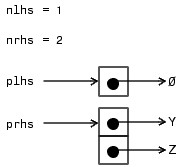
\includegraphics[width=0.4\textwidth]{../../img/20151110mexinputoutput.jpg}
\caption{\label{fig:orgparagraph1}
mexFunction输入输出参数}
\end{figure}

由于输入参数是两个,所以 \texttt{mexFunction} 的 \texttt{nrhs=2} ; 由于输出参数是2个, 所以 \texttt{mexFunction} 的 \texttt{nlhs=2} 。输入参数通过指针数组 \texttt{prhs} 来索引: \texttt{prhs[0]} 指向 \texttt{Y} ; \texttt{prhs[1]} 指向 \texttt{Z} 。输出参数通过指针 \texttt{plhs} 来获取,调用 \texttt{mexFunction} 时,该指针为空指针,我们需要在 \texttt{myFunction.c} 里面为其申请空间,并赋予 \texttt{plhs[0]} 和 \texttt{plhs[1]} 申请的内存空间地址(这一步是很重要的,再说一遍:在我们编写 \texttt{myFunction.c} 时需要在 \texttt{mexFunction} 函数体内为 \texttt{plhs[0]} 和 \texttt{plhs[1]} 赋予一个地址,指向存放输出的内存地址)。
\subsection{\texttt{mexFunction} 的数据流动}
\label{sec:orgheadline9}


当我们调用 \texttt{[C,D]=func[A,B]} 时, 图\ref{fig:orgparagraph2}给出了输入输出的转换过程。
\begin{figure}[htb]
\centering
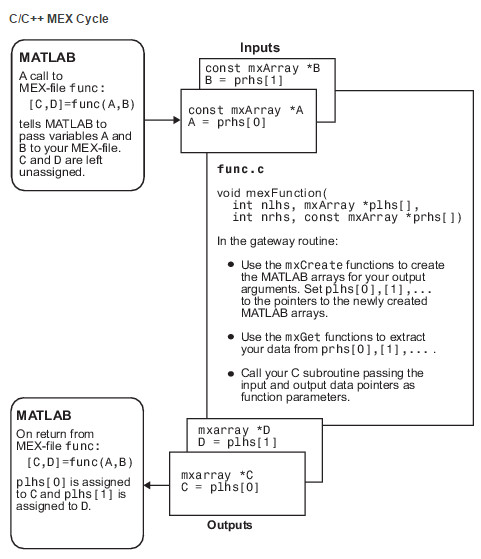
\includegraphics[width=0.6\textwidth]{../../img/20151110mexdataflow.jpg}
\caption{\label{fig:orgparagraph2}
调用[C,D]=func[A,B]对应的数据流程}
\end{figure}

整个过程大致可以用以下步骤描述:
\begin{enumerate}
\item matlab脚本调用 \texttt{[C,D]=func[A,B]} ,把 \texttt{A,B} 作为输入传送给 MEX文件, \texttt{C,D} 未赋值。 ( 注意这一步是matlab自动为我们完成的。)
\item 在 \texttt{mexFunction} 函数里, 通过 \texttt{A=prhs[0]} 和 \texttt{B=prhs[1]} 获取指向输入的地址。( 注意这一步是需要我们自己完成的)
\item 使用 \texttt{mxCreate} 函数创建用于保存输出的数组,并把这些数组的地址赋给 \texttt{plhs[0]} 和 \texttt{plhs[1]} ( 注意这一步是需要我们自己完成的)
\item 在matlab脚本中, MEX文件的返回值通过 \texttt{plhs[0]} 和 \texttt{plhs[1]} 赋给 \texttt{C,D} 。(注意这一步是matlab自动为我们完成的。)
\end{enumerate}

在上述步骤2和步骤3中,matlab为我们提供了很多API方便我们对输入和输出进行操作,比如\hyperref[orgtarget1]{创建桥梁变量} 一节用到的 \texttt{mxGetN} 等函数,还有这一节用到的 \texttt{mxCreate} 函数。这些API是matlab提供的。通过 \texttt{\#include “mex.h”} 我们可以在自己的C文件中使用,就像使用C语言自带的函数库一样。
\section{尾声}
\label{sec:orgheadline11}


matlab调用C函数要点
\begin{itemize}
\item matlab使用 \texttt{mexFunction} 封装用户定义的C函数
\item 用户使用matlab调用C函数(这里是 \texttt{arrayProduct} )就像调用matlab的内嵌函数一样。对用户来讲, \texttt{mexFunction} 是透明的,就像不存在一样。
\item matlab脚本和 \texttt{mexFunction} 之间使用 \texttt{nlhs} \texttt{plhs} \texttt{nrhs} \texttt{prhs} 来完成参数传递。 \texttt{mexFunction} 函数使用matlab提供的API实现参数传递和matlab数据类型到C数据类型的转换。
\item matlab 使用 \texttt{mex} 命令将用户编写的C文件编译成后缀名为 \texttt{mexw64} 的文件(后缀名依操作系统而定)。
\end{itemize}
\end{document}
